The translation factor is the ratio between the signal region yield and single lepton control sample yield in the simulation samples (\ttbar, $W$+jets and single top). The translation factor method is straightforward to apply. First, we calculate the translation factors for each search bin in the single lepton control sample in simulation events. The simulation events are corrected to account for residual differences with respect to data with ISR-reweighting, b-jet tag efficiencies and lepton reconstruction efficiencies. Then, we apply those factors to the single lepton control samples in data to estimate the backgrounds. The translation factors for misidentified leptons (lost lepton) and decaying tau leptons are shown in Figs~\ref{fig:hadtau_TF} and \ref{fig:lostle_TF}, for the single muon and electron control samples respectively. The final prediction combines the results from the single electron and single muon samples together (Figs~\ref{fig:TAUpredictionSB} and \ref{fig:LLpredictionSB}). 

\begin{figure}[htbp]
  \begin{center}
  \begin{tabular}{c}
  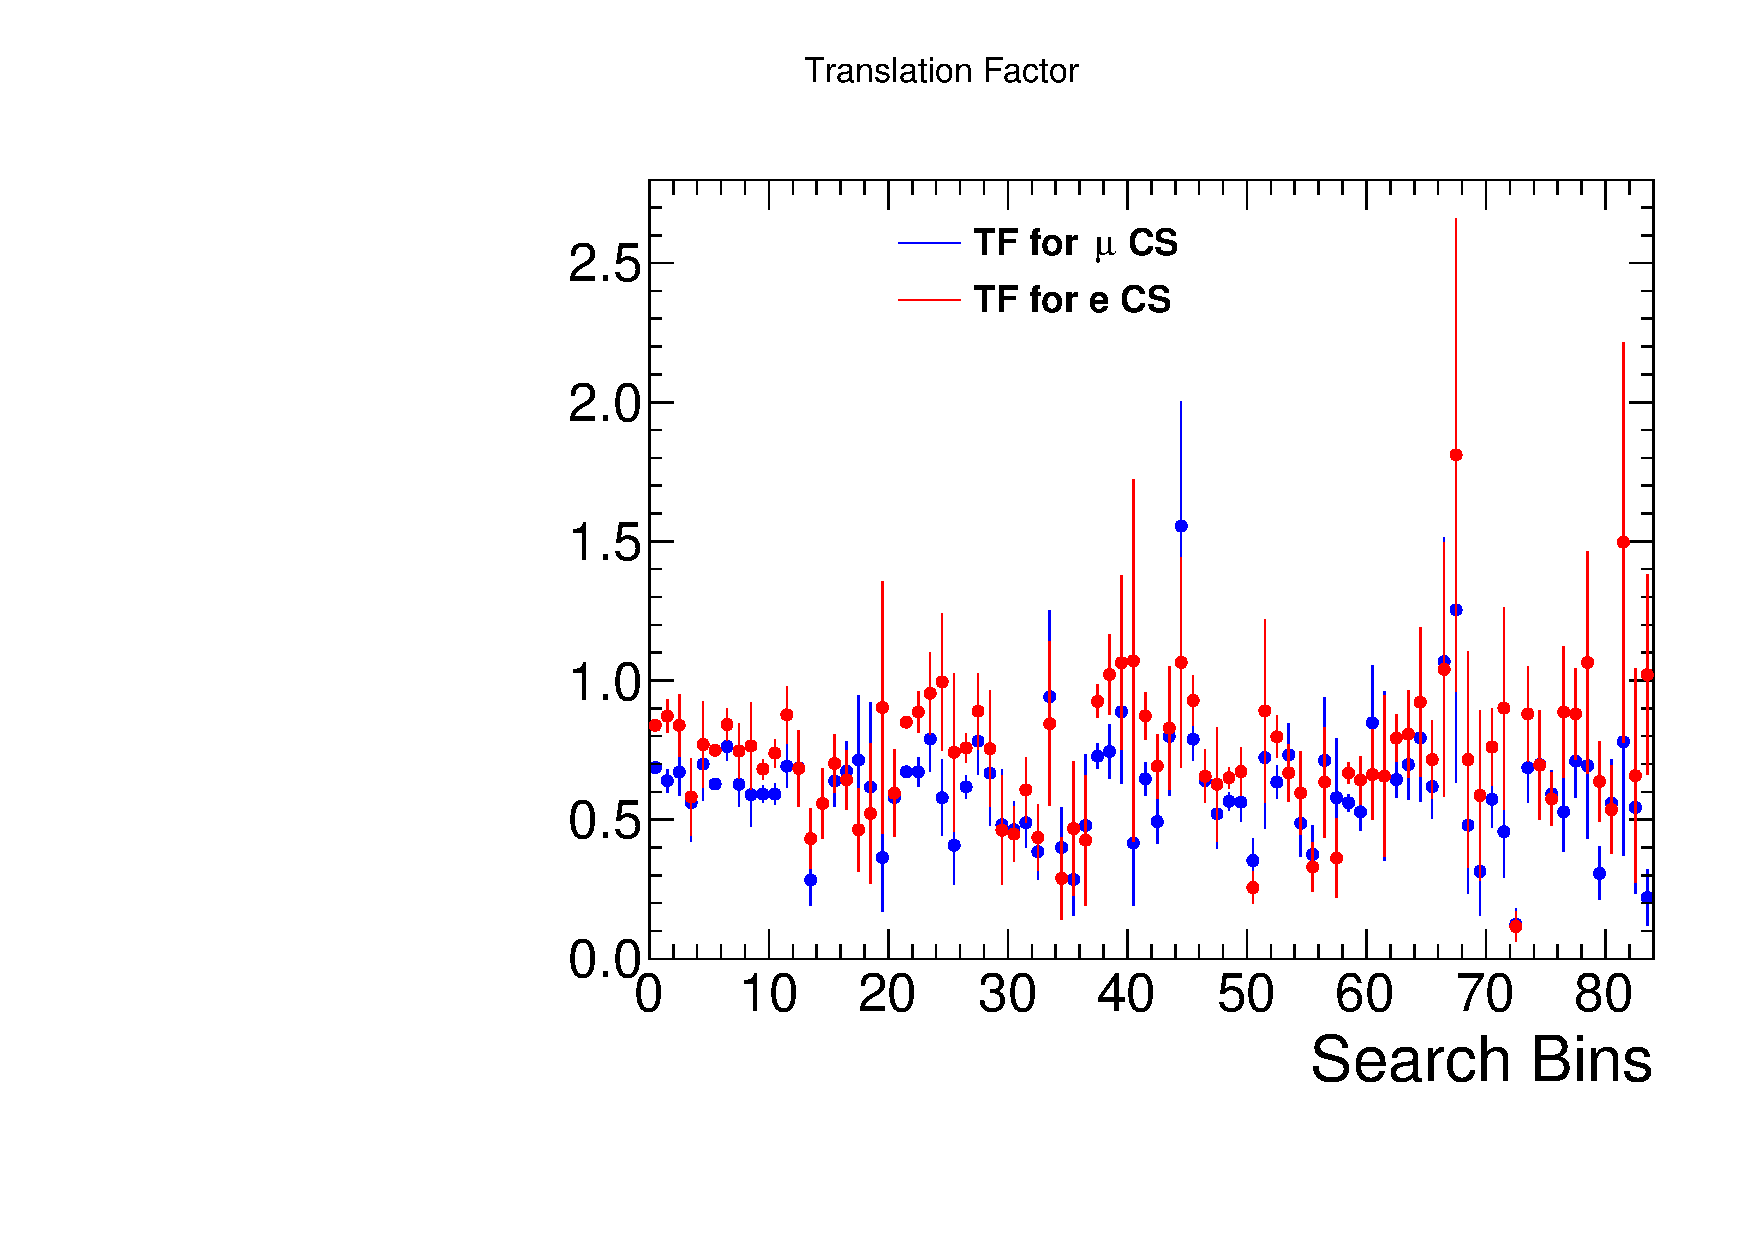
\includegraphics[angle=0,width=0.60\textwidth]{sections/mc4/Backgrounds/TF/figures/comp_TF_hadtau_comb.pdf}
  \end{tabular}
  \caption{Translation factors for the \tauh background prediction with their uncentainties from limited MC statistics for both muon and electron CS}
    \label{fig:hadtau_TF}
  \end{center}
\end{figure}


\begin{figure}[htbp]
  \begin{center}
  \begin{tabular}{c}
  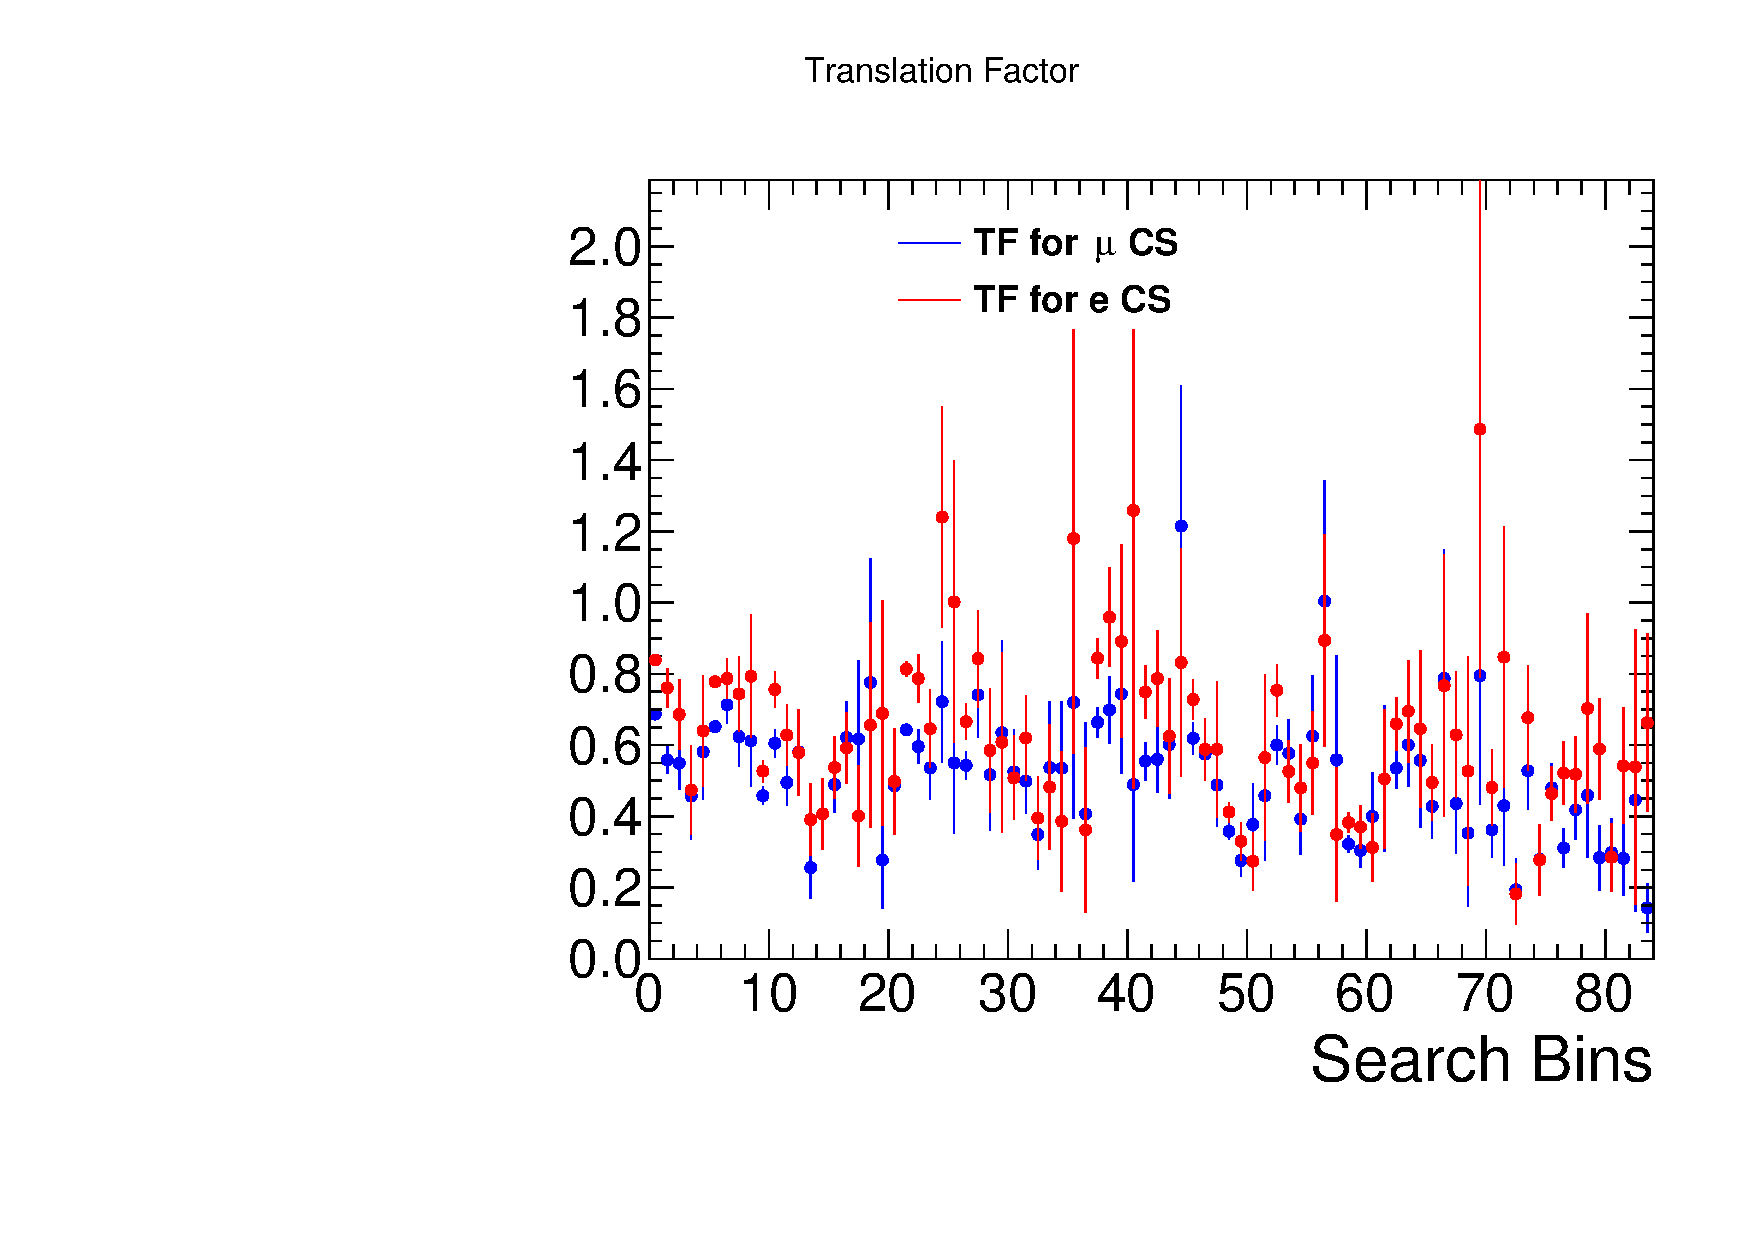
\includegraphics[angle=0,width=0.60\textwidth]{sections/mc4/Backgrounds/TF/figures/comp_TF_lostle_comb.pdf}
  \end{tabular}
  \caption{Translation factors for the lost lepton background prediction with their uncentainties from limited MC statistics for both muon and electron CS}
    \label{fig:lostle_TF}
  \end{center}
\end{figure}

\begin{figure}[htbp]
  \begin{center}
  \begin{tabular}{cc}
  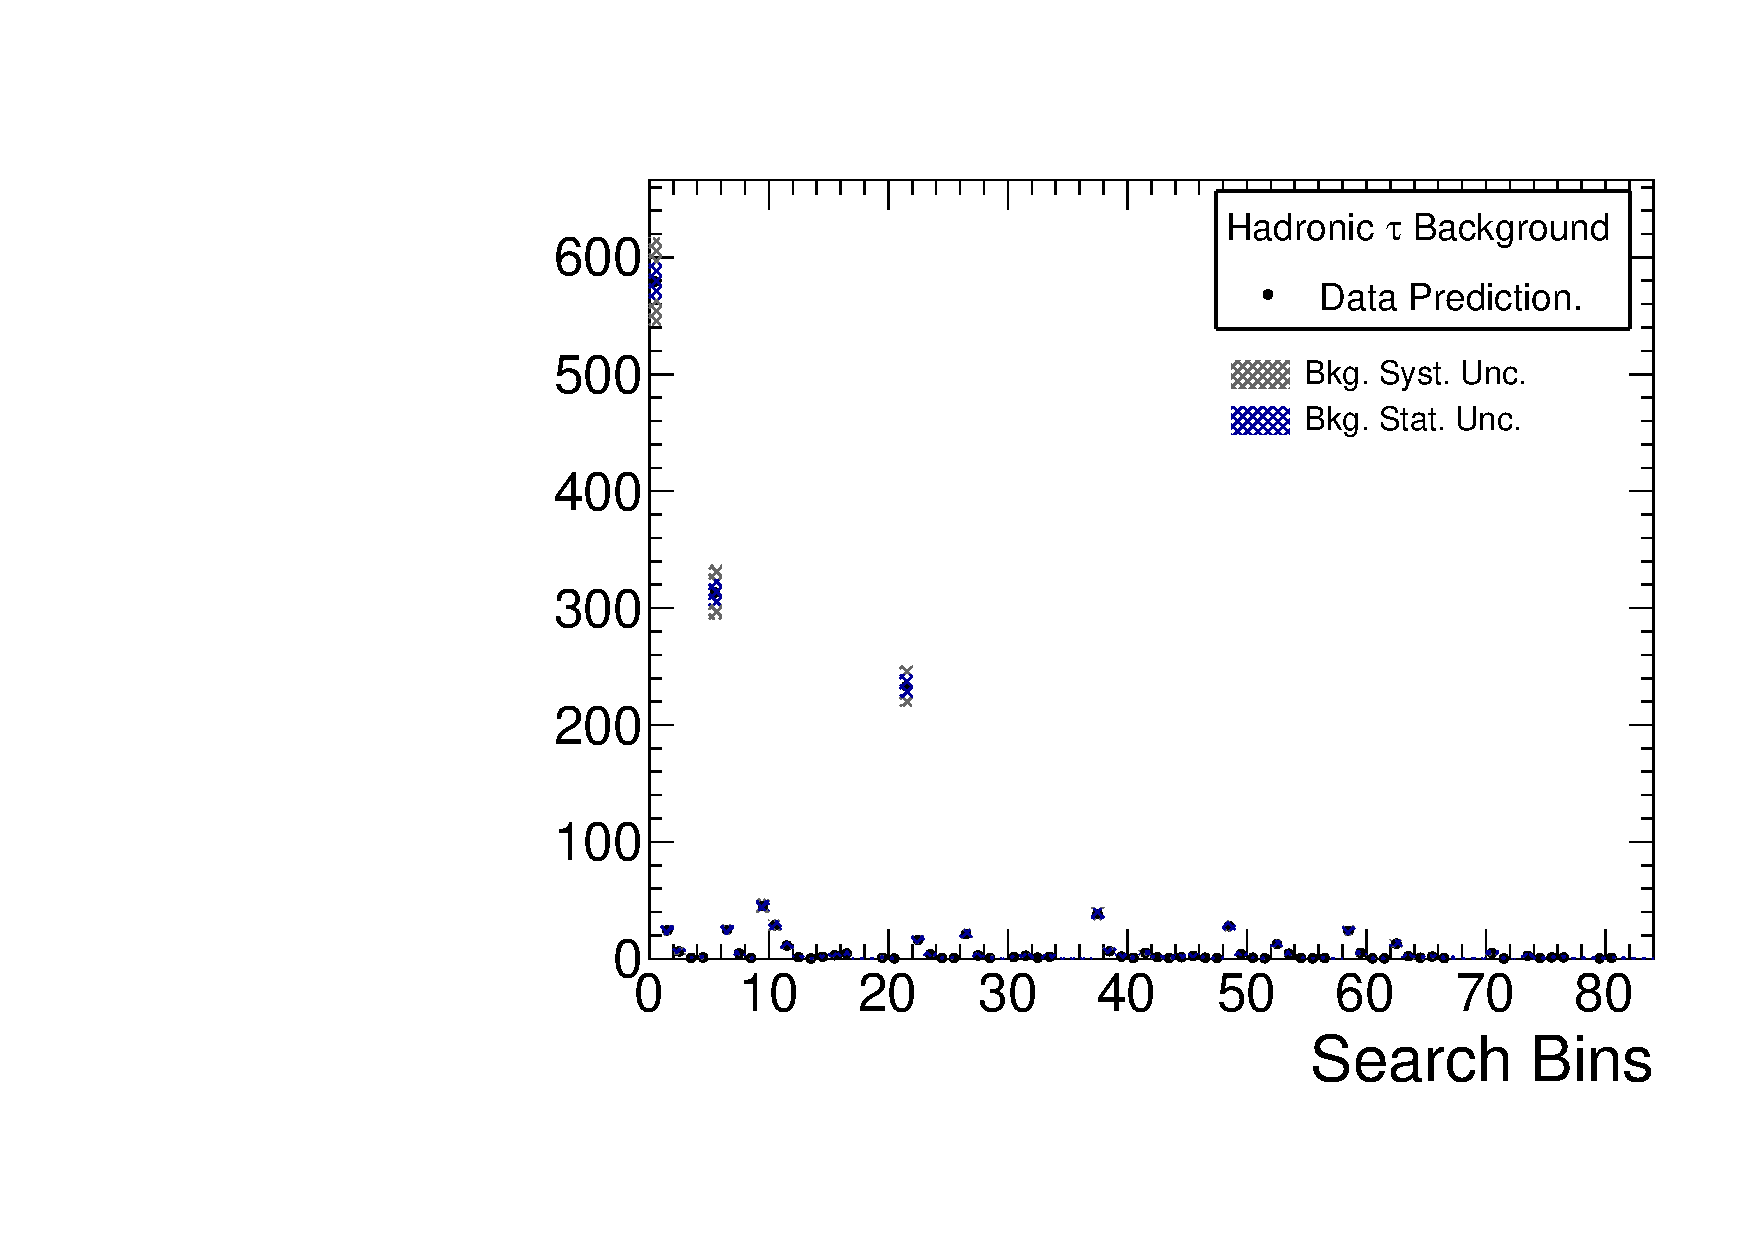
\includegraphics[angle=0,width=0.5\textwidth]{sections/mc4/Backgrounds/TF/figures/pred_full_hadtau_comb.pdf}
  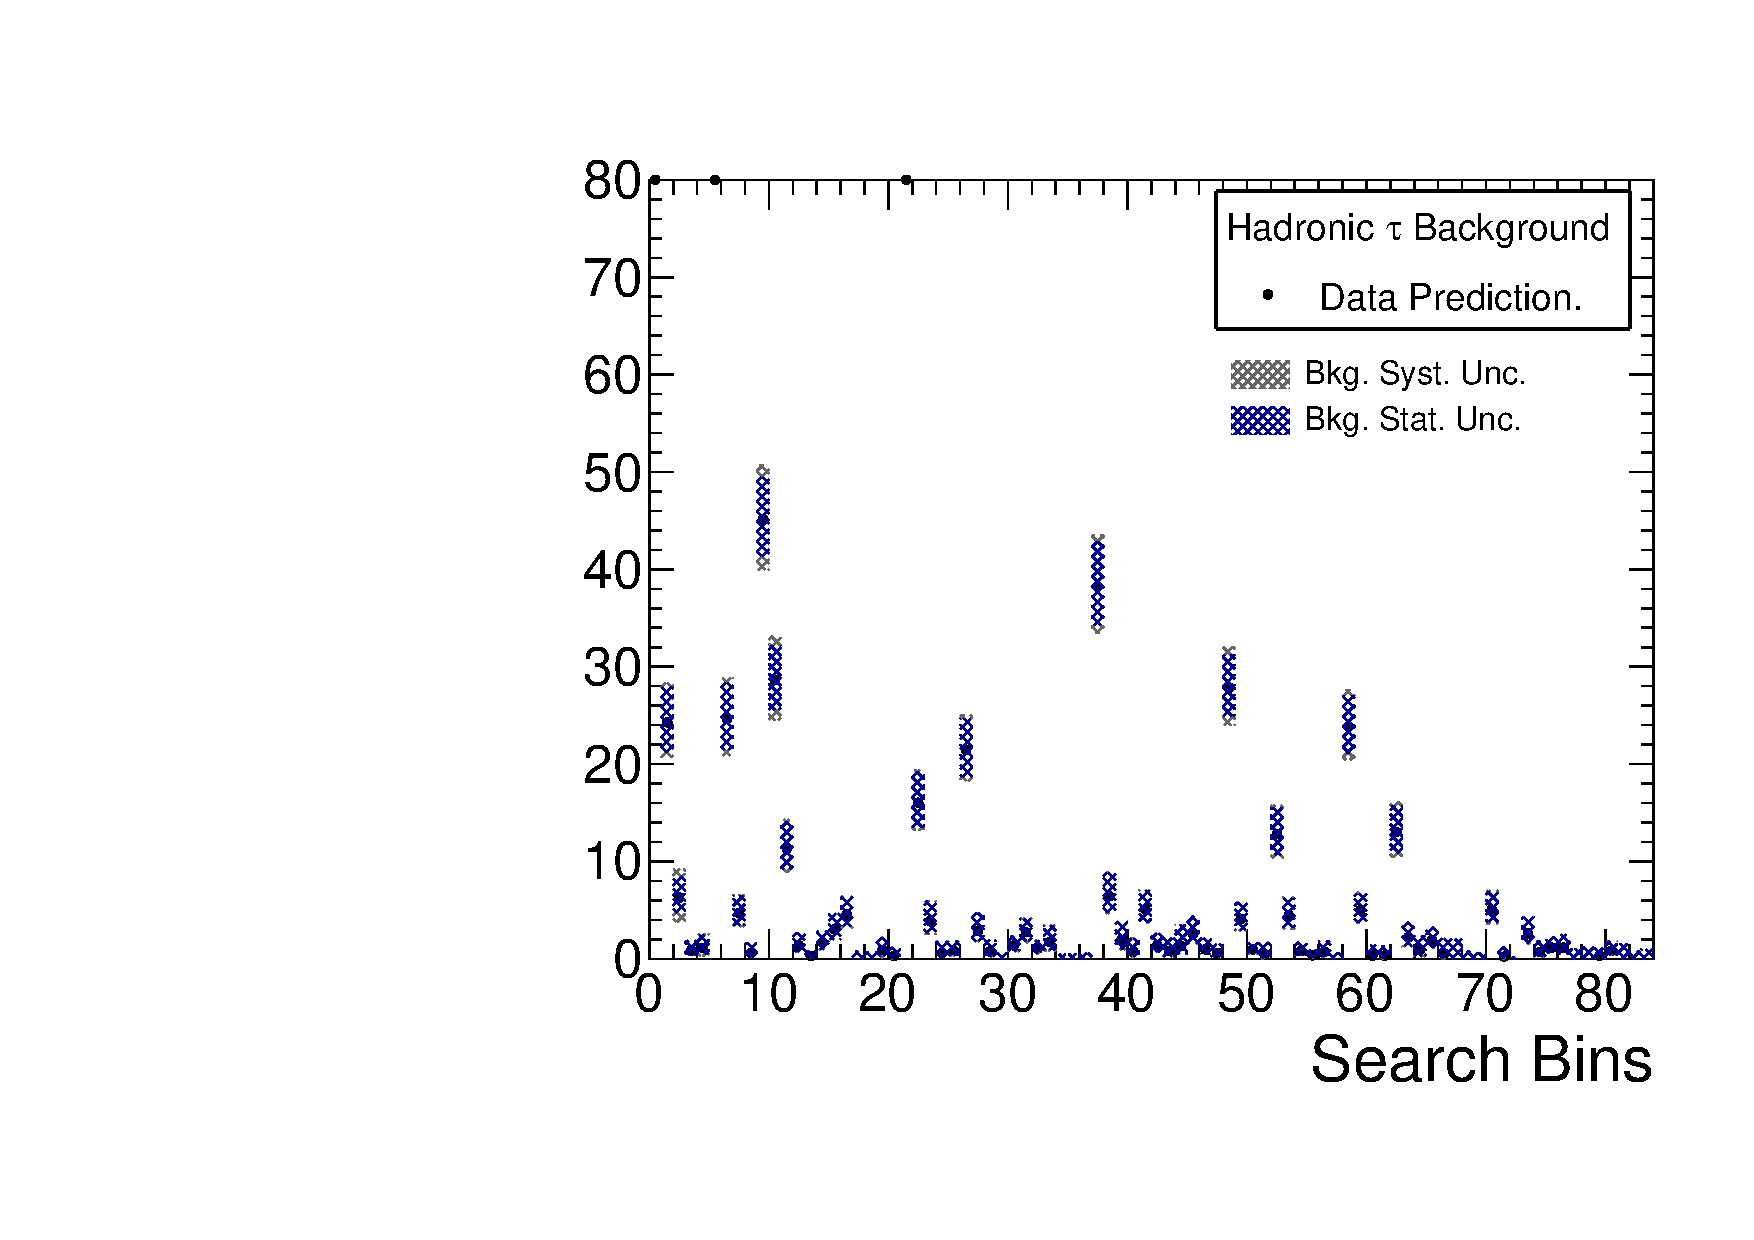
\includegraphics[angle=0,width=0.5\textwidth]{sections/mc4/Backgrounds/TF/figures/pred_zoomin_hadtau_comb.pdf}
  \end{tabular}
  \caption{Predicted hadronic tau background yield for a $35.9$~fb$^{-1}$ data for all the search regions. Right plot is a zoomed version of left plot.
Both statistical and total systematic uncertainties are shown. }
    \label{fig:TAUpredictionSB}
  \end{center}
\end{figure}

\begin{figure}[htbp]
  \begin{center}
  \begin{tabular}{cc}
  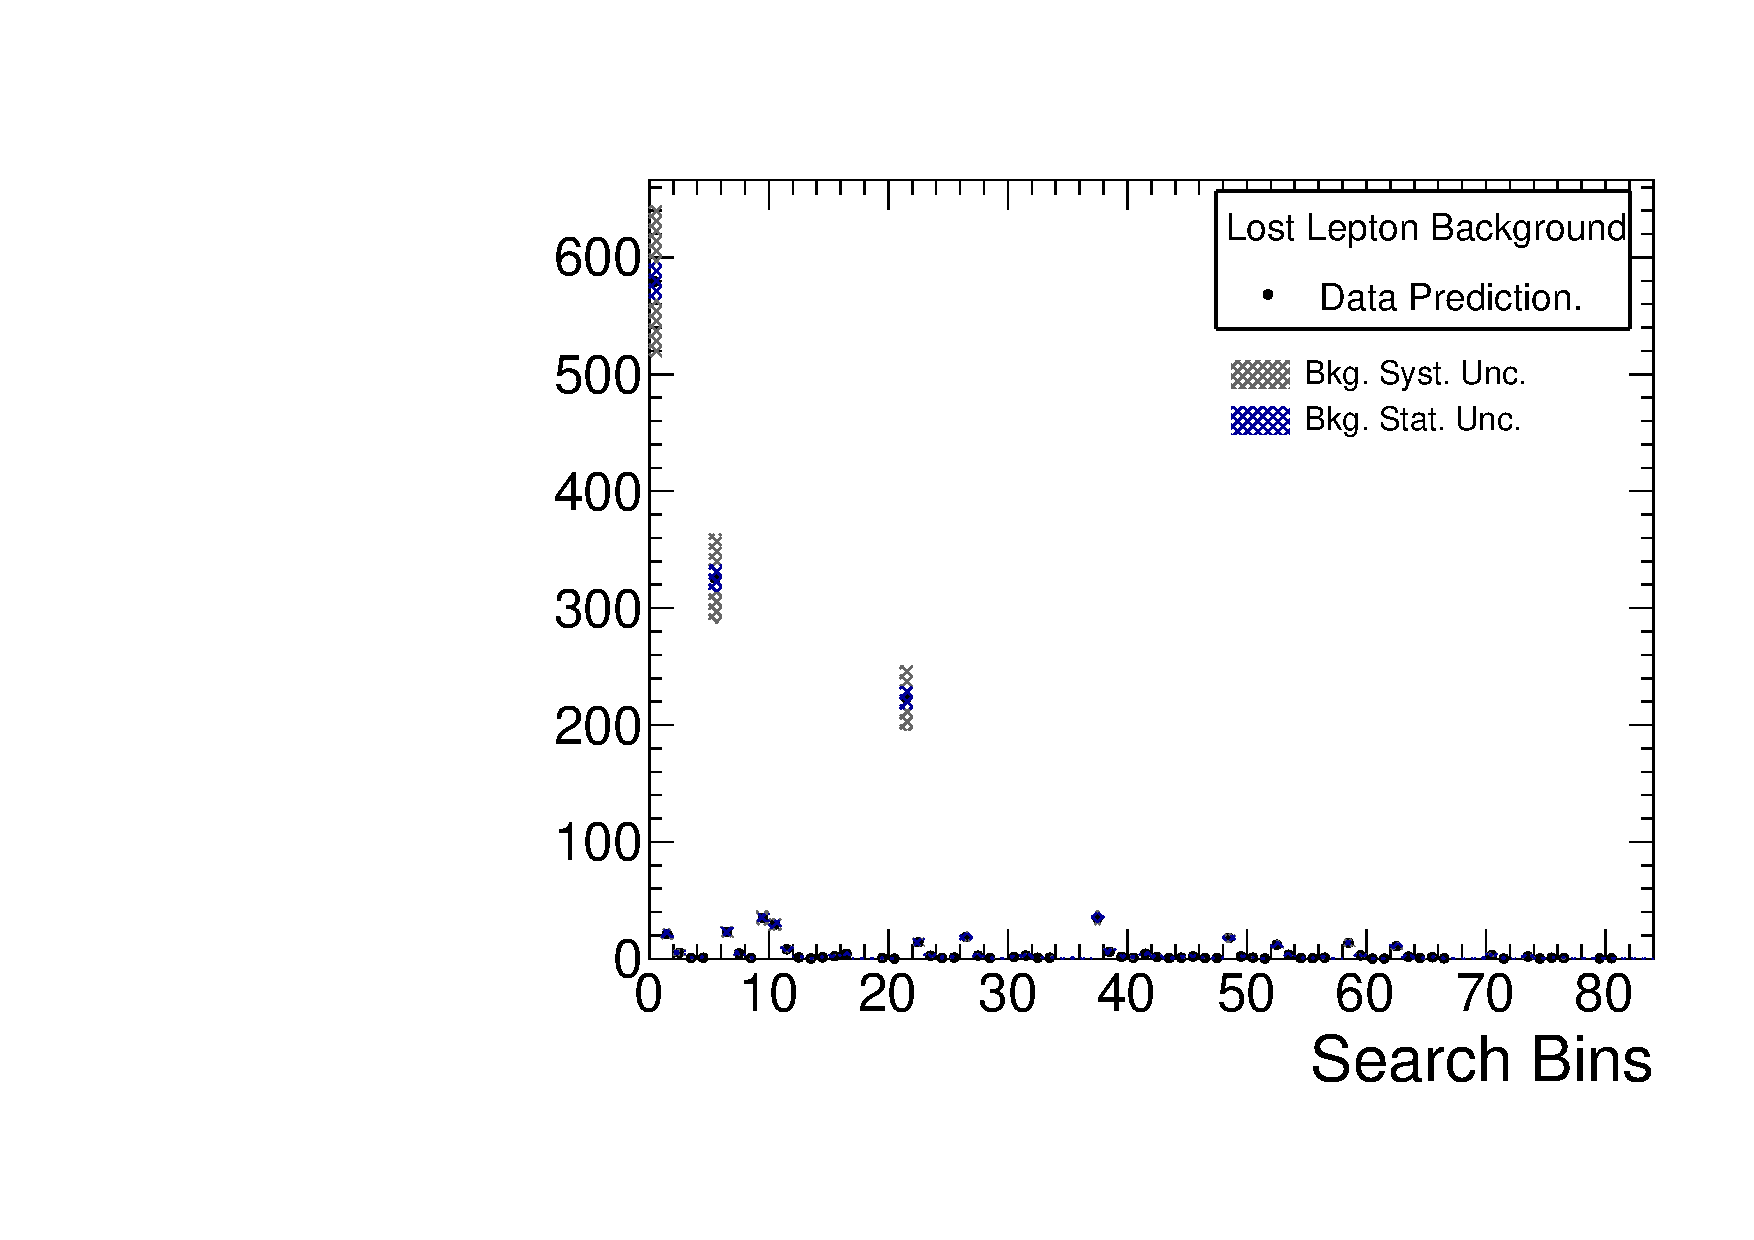
\includegraphics[angle=0,width=0.5\textwidth]{sections/mc4/Backgrounds/TF/figures/pred_full_lostle_comb.pdf}
  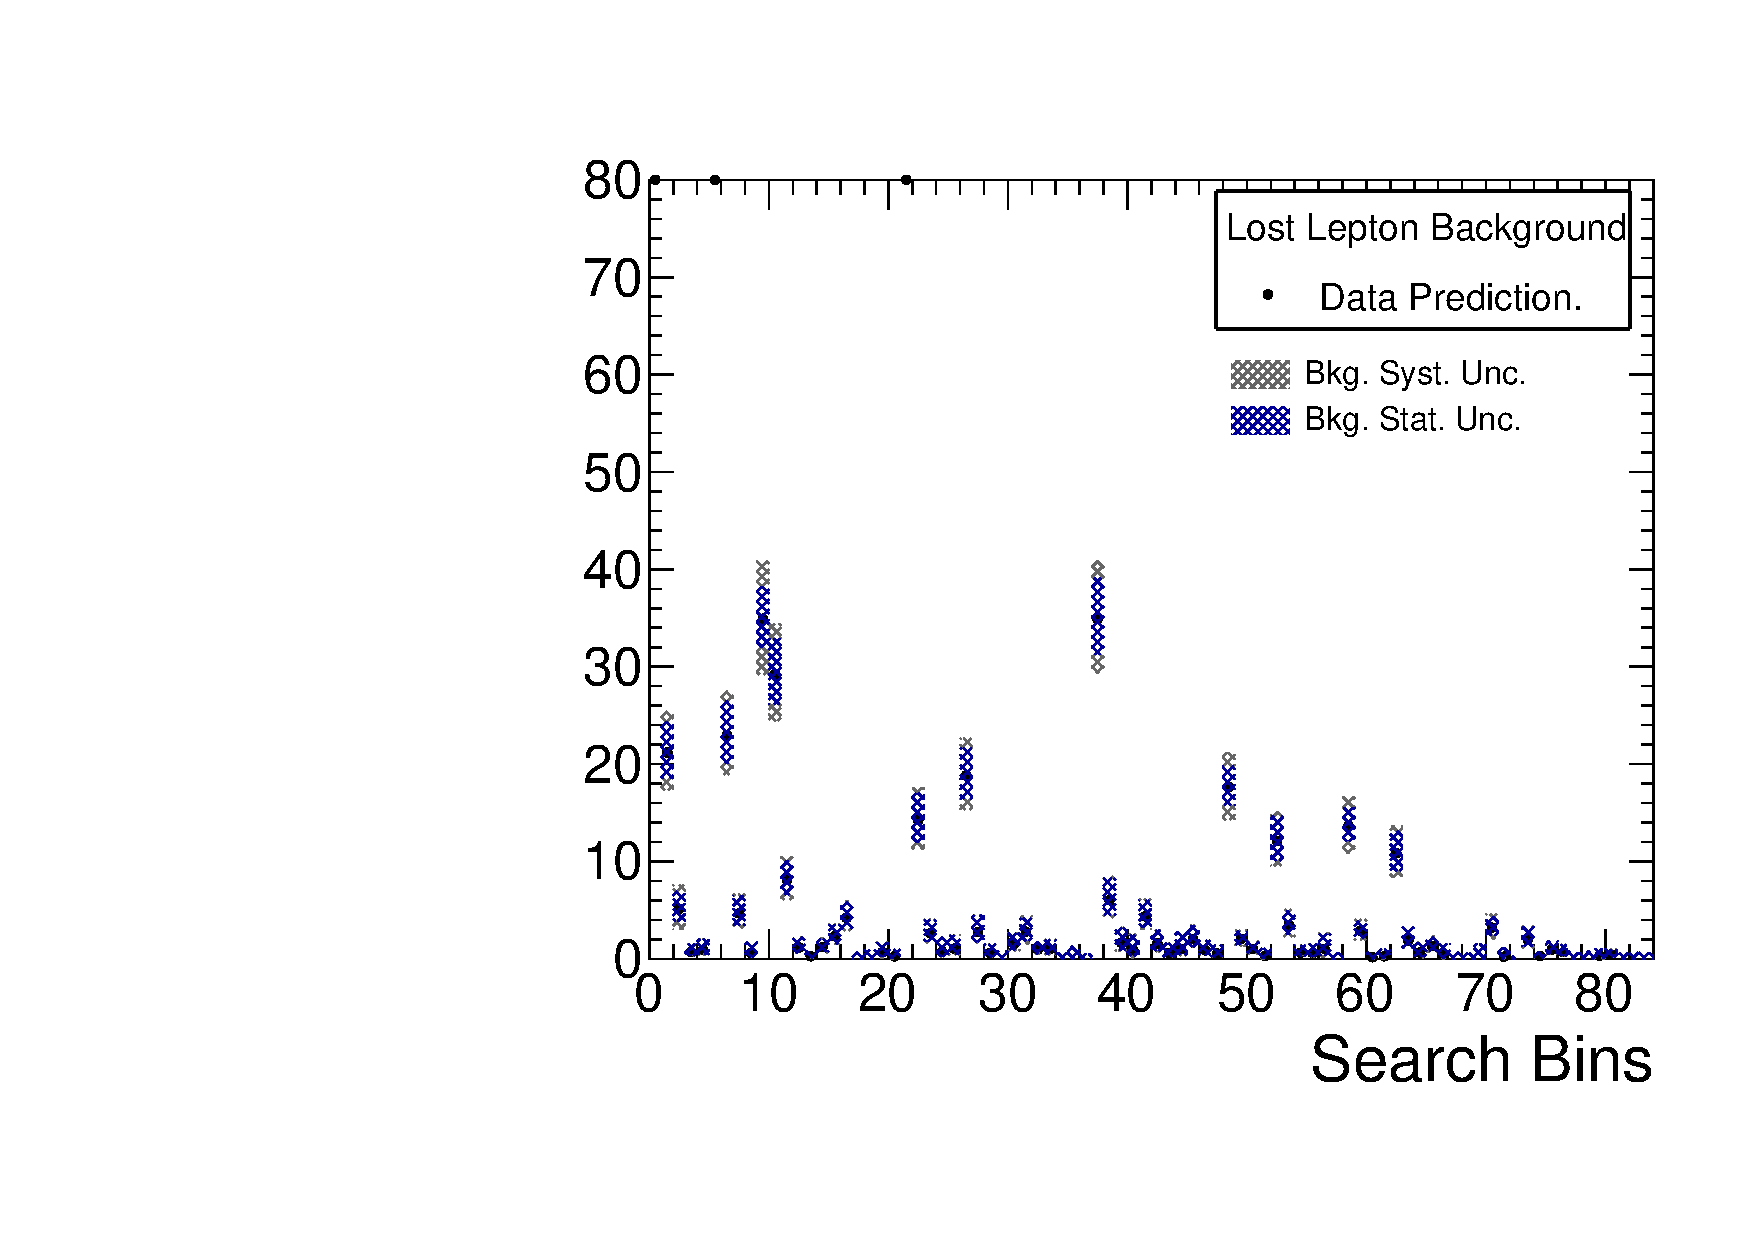
\includegraphics[angle=0,width=0.5\textwidth]{sections/mc4/Backgrounds/TF/figures/pred_zoomin_lostle_comb.pdf}
  \end{tabular}
  \caption{Predicted lost lepton background yield for a $35.9$~fb$^{-1}$ data for all the search regions. Right plot is a zoomed version of left plot.
Both statistical and total systematic uncertainties are shown. }
    \label{fig:LLpredictionSB}
  \end{center}
\end{figure}
